\chapter{Preliminaries}

\section{System Model}
We assume a system consisting of a set P of computing nodes and a set L of bidirectional communication links between nodes. L consists of one link for each unordered pair of nodes, i.e., every possible link is represented. The nodes are assumed to be completely reliable. The links between nodes go up and down, due to the movement of the nodes. While a link is up, the communication across it is in first-in-first-out order and is reliable but asynchronous.

We model the whole system as a set of (infinite) state machines that interact through shared events (a specialization of the IOA model [12]). Each node and each link is modeled as a separate state machine. The shared events are Link Up/Down notifications and receipt of messages, all of which are controlled and initiated by the link and responded to by the node. The sending of a message is also a shared event, but it is controlled and initiated by the node and responded to by the link; we are not explicitly modeling this.

The next subsection gives more details about how links are modeled and specifies the initial states. The algorithm executed by the nodes and its initial states are described in Section 3.
\section{Modeling Asynchronous Dynamic Links}
We now specify how communication is assumed to occur over the dynamic links, and how notification of a link’s status is synchronized at the two endpoints of the link.

The state of a link Link{u, v}, which models the bidirectional communication link between node u and node v, consists of a status variable and two queues of messages.

The possible values of the status variable are Up, GoingDown u , GoingDown v , Down, ComingUp u , and ComingUp v . The link transitions among different values of its status variable through LinkUp and LinkDown events. Figure 1 shows the state transition diagram for Link{u, v}. The intuition is that if a LinkUp (resp., LinkDown) occurs at one endpoint of the link, then LinkUp (resp., LinkDown) must occur at the other endpoint before LinkDown (resp., LinkUp) can occur at either end.

The other components of the link’s local state are the two message queues: mqueue u,v holds messages in transit from u to v and mqueue v,u holds messages in transit from v to u.

An attempt by node u to send a message to node v results in the message being appended to mqueue u,v if the link’s status is either ComingUp u or Up; otherwise there is no effect.
\begin{figure}[hbtp]
\centering
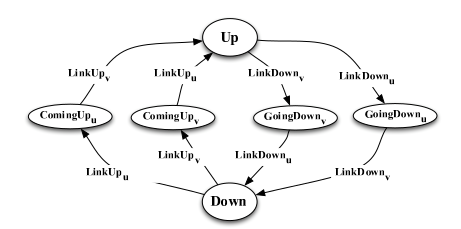
\includegraphics[scale=.75]{screenshot.png}
\caption{State diagram for status variable of $Link\lbrace u, v\rbrace$ .}
\end{figure}

If the status is ComingUp u , then messages in transit from u to v are held in the queue until v has been notified that the link is Up. Once the link is Up, the event by which node u receives the message at the head of mqueue v,u is enabled to occur. An attempt by node v to send a message to node u is handled analogously.

Whenever a LinkDown u or LinkDown v event occurs, both message queues are emptied. Neither u nor v is alerted to which messages in transit have been lost due to the LinkDown.

In an initial state of the link, both message queues are empty and the status is either Up or Down.
\section{Configurations and Executions}
The notion of configuration is used to capture an instan-
taneous snapshot of the state of the entire system. A config-
uration is a vector of node states, one for each node in P,
and a vector of link states, one for each link in L .
Assume that the undirected graph G = (V, E) defines the
initial communication topology of the system, where V is a
set of vertices corresponding to the set P of nodes, and E
is a set of edges corresponding to the set of communication
links that are up. In an initial configuration with respect
to G, each node is in an initial state (as prescribed by the
node’s algorithm), each link corresponding to an edge in E
is in an initial state with its status equal to Up, and every
other link has its status equal to Down.
Define an execution as an infinite sequence
C 0 , e 1 ,C 1 , e 2 ,C 2 , . . . of alternating configurations and
events, starting with an initial configuration and, if finite,
ending with a configuration, that satisfies the following
safety conditions:
\begin{itemize}
\item C 0 is an initial configuration (w.r.t. some initial topology G).
\item The preconditions for event are true in $C_{i-1}$ for all $i\geq 1$.
\item C i is the result of executing event e i on configuration C i−1 , for all i ≥ 1 (only the node and link involved in an event change state, and they change according to their state machine transitions).
\end{itemize}

An execution also satisfies the following liveness condi-
tions:
\begin{itemize}
\item If a link remains Up for infinitely long, then every message sent over the link is eventually delivered.
\item For each link, if only a finite number of link events occur, then the link status after the last one is either Up or Down (not in between).
\end{itemize}

We also assign a positive real-valued global time gt to each event e i , i ≥ 1, such that gt(e i ) < gt(e i+1 ) and, if the execution is infinite, the global times increase without bound. Each configuration inherits the global time of its preceding event, so gt(C i ) = gt(e i ) for i ≥ 1; we define gt(C 0 ) to be 0. We assume that the nodes do not have access to gt.
\section{Problem Definition}
Each node u in the system has a local variable lid u to hold the identifier of the node currently considered by u to be the leader of the connected component containing u.

In every execution that includes a finite number of topology changes, we require that the following eventually holds:
Every connected component CC of the final topology contains a node l, the leader, such that lid u = l for all nodes $u \in CC$, including l itself.

Our algorithm also ensures that eventually each link in the system has a direction imposed on it by virtue of the data stored at each endpoint such that each connected component CC is a leader-oriented DAG, i.e., every node has a directed path to the leader.
